% Generated by ArticleSignalDiagrams. Opaque vector fills only.
\documentclass[10pt,tikz,border=5pt]{standalone}
\usepackage{lmodern}
\usetikzlibrary{fit}
\begin{document}
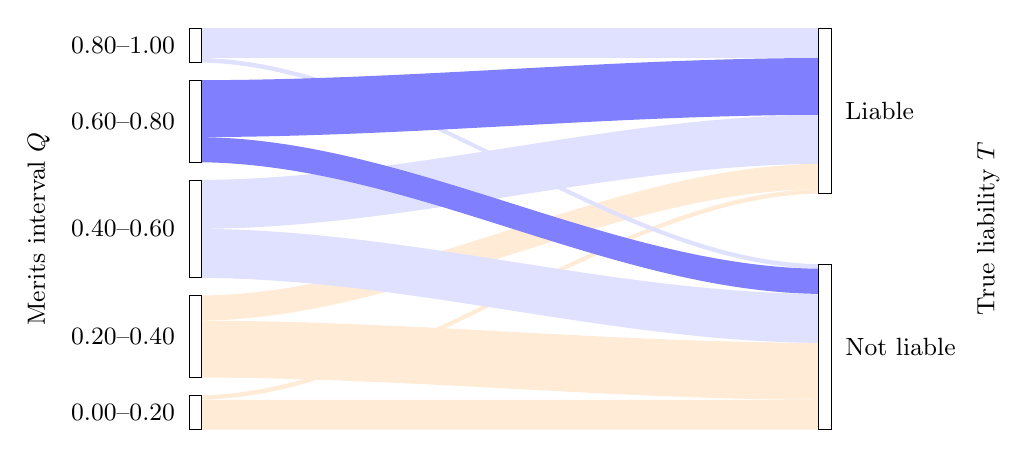
\begin{tikzpicture}[x=1cm,y=1cm,font=\small]\path[fill=orange!16!white,draw=none] (3.3,-5.1) .. controls (6,-5.1) and (8.6,-5.1) .. (11.3,-5.1) -- (11.3,-4.72032) .. controls (8.6,-4.72032) and (6,-4.72032) .. (3.3,-4.72032) -- cycle;
\path[fill=orange!16!white,draw=none] (3.3,-4.72032) .. controls (6,-4.72032) and (8.6,-2.1) .. (11.3,-2.1) -- (11.3,-2.04288) .. controls (8.6,-2.04288) and (6,-4.6632) .. (3.3,-4.6632) -- cycle;
\path[fill=orange!16!white,draw=none] (3.3,-4.4382) .. controls (6,-4.4382) and (8.6,-4.72032) .. (11.3,-4.72032) -- (11.3,-3.99792) .. controls (8.6,-3.99792) and (6,-3.7158) .. (3.3,-3.7158) -- cycle;
\path[fill=orange!16!white,draw=none] (3.3,-3.7158) .. controls (6,-3.7158) and (8.6,-2.04288) .. (11.3,-2.04288) -- (11.3,-1.72368) .. controls (8.6,-1.72368) and (6,-3.3966) .. (3.3,-3.3966) -- cycle;
\path[fill=blue!12!white,draw=none] (3.3,-3.1716) .. controls (6,-3.1716) and (8.6,-3.99792) .. (11.3,-3.99792) -- (11.3,-3.37632) .. controls (8.6,-3.37632) and (6,-2.55) .. (3.3,-2.55) -- cycle;
\path[fill=blue!12!white,draw=none] (3.3,-2.55) .. controls (6,-2.55) and (8.6,-1.72368) .. (11.3,-1.72368) -- (11.3,-1.10208) .. controls (8.6,-1.10208) and (6,-1.9284) .. (3.3,-1.9284) -- cycle;
\path[fill=blue!12!white,draw=none] (3.3,-0.4368) .. controls (6,-0.4368) and (8.6,-3.05712) .. (11.3,-3.05712) -- (11.3,-3) .. controls (8.6,-3) and (6,-0.37968) .. (3.3,-0.37968) -- cycle;
\path[fill=blue!12!white,draw=none] (3.3,-0.37968) .. controls (6,-0.37968) and (8.6,-0.37968) .. (11.3,-0.37968) -- (11.3,-0) .. controls (8.6,-0) and (6,-0) .. (3.3,-0) -- cycle;
\path[fill=blue!50!white,draw=none] (3.3,-1.7034) .. controls (6,-1.7034) and (8.6,-3.37632) .. (11.3,-3.37632) -- (11.3,-3.05712) .. controls (8.6,-3.05712) and (6,-1.3842) .. (3.3,-1.3842) -- cycle;
\path[fill=blue!50!white,draw=none] (3.3,-1.3842) .. controls (6,-1.3842) and (8.6,-1.10208) .. (11.3,-1.10208) -- (11.3,-0.37968) .. controls (8.6,-0.37968) and (6,-0.6618) .. (3.3,-0.6618) -- cycle;
\coordinate (axis-midline-0) at (0,-2.55);
\path[fill=white,draw=black,line width=0.3pt] (3.22,-5.1) rectangle (3.38,-4.6632);
\node[anchor=east,fill=white,inner sep=2pt] (bucket-0-0-0) at (3.12,-4.8816) {0.00--0.20};
\path[fill=white,draw=black,line width=0.3pt] (3.22,-4.4382) rectangle (3.38,-3.3966);
\node[anchor=east,fill=white,inner sep=2pt] (bucket-0-0-1) at (3.12,-3.9174) {0.20--0.40};
\path[fill=white,draw=black,line width=0.3pt] (3.22,-3.1716) rectangle (3.38,-1.9284);
\node[anchor=east,fill=white,inner sep=2pt] (bucket-0-0-2) at (3.12,-2.55) {0.40--0.60};
\path[fill=white,draw=black,line width=0.3pt] (3.22,-1.7034) rectangle (3.38,-0.6618);
\node[anchor=east,fill=white,inner sep=2pt] (bucket-0-0-3) at (3.12,-1.1826) {0.60--0.80};
\path[fill=white,draw=black,line width=0.3pt] (3.22,-0.4368) rectangle (3.38,-0);
\node[anchor=east,fill=white,inner sep=2pt] (bucket-0-0-4) at (3.12,-0.2184) {0.80--1.00};
\node[fit=(bucket-0-0-0) (bucket-0-0-1) (bucket-0-0-2) (bucket-0-0-3) (bucket-0-0-4),inner sep=0pt] (source-labels-0) {};
\coordinate (axis-title-0-0) at (source-labels-0.west |- axis-midline-0);
\node[rotate=90,anchor=south,inner sep=0pt] at ([xshift=-0.18cm]axis-title-0-0) {Merits interval $Q$};
\path[fill=white,draw=black,line width=0.3pt] (11.22,-5.1) rectangle (11.38,-3);
\node[anchor=west,fill=white,inner sep=2pt] (bucket-0-1-0) at (11.48,-4.05) {Not liable};
\path[fill=white,draw=black,line width=0.3pt] (11.22,-2.1) rectangle (11.38,-0);
\node[anchor=west,fill=white,inner sep=2pt] (bucket-0-1-1) at (11.48,-1.05) {Liable};
\node[fit=(bucket-0-1-0) (bucket-0-1-1),inner sep=0pt] (destination-labels-0) {};
\coordinate (axis-title-0-1) at (destination-labels-0.east |- axis-midline-0);
\node[rotate=90,anchor=north,inner sep=0pt] at ([xshift=0.18cm]axis-title-0-1) {True liability $T$};
\end{tikzpicture}
\end{document}

